\chapter{Projeto de implementação}
\label{cap:projetoimplementacao}

Neste capítulo será feita a definição das ferramentas que irão compor o ambiente de alta disponibilidade. A solução será baseada na utilização 
de virtualização e de \textit{softwares} de código aberto, e será descrita na Seção \ref{section:implementacao}.

\section{Definição dos softwares utilizados}
\label{section:propostasolucao}

Usar metodologia MAH Método Analítico Hierárquico \cite{geordano2014} ?? detalhar metodologia ??
%Para comparar e selecionar o \textit{software} mais adequado para esta implementação utilizou-se uma técnica semelhante à descrita no artigo 
%de \cite{thome2013}. Neste artigo foi feita uma análise comparativa de ferramentas \textit{open source} de computação em nuvem. Sendo que, 
%foram criadas as seguintes características para fazer uma análise comparativa das ferramentas:
%interface, gerenciamento de energia, balanceamento de carga, rede, armazenamento, monitoramento, integração, virtualização, segurança, 
%escalabilidade e tolerância a falhas. Essas características são importantes para medir a qualidade e compatibilidade das ferramentas estudadas, 
%além de comparar a usabilidade das ferramentas.

Com base neste artigo, procurou-se selecionar as características mais relevantes para o real ambiente existente e compatível com o projeto 
de implementação. 
Além disso, dois tipos de \textit{softwares} foram necessários para a implementação da alta disponibilidade, estes foram divididos em dois grupos: 
\textit{softwares} de replicação de dados; e \textit{softwares} para o monitoramento e gerência do \textit{cluster} (transferências das máquinas 
virtuais entre os nós). As características que serão utilizadas para adotar o \textit{software} mais adequado para a implementação deste 
trabalho estão listadas abaixo.
%Foram consideradas as características, funcionalidades e formas de operação, para possibilitar a comparação das ferramentas.

\textit{Software} de replicação de dados:
\begin{itemize}
 \item Integração com virtualização;
 \item Dual-primary;
 \item Replicação em tempo real;
 \item Nível de replicação;
 \item Número máximo de nós.
\end{itemize}

\textit{Software} para monitoramento e gerência do \textit{cluster}:
\begin{itemize}
 \item Suporte nativo a virtualização;
 \item Migração de \acp{VM} em tempo real;
 \item Failover e failback automáticos;
 \item Sincronismo de configuração entre os nós.
\end{itemize}

\subsection{Softwares para a replicação de dados}
\label{section:toolrepl}

A replicação de dados pode ser realizada de diferentes formas, esta pode ser a nível de aplicação ou até mesmo a nível de \textit{hardware}.
Dependendo do objetivo pode-se utilizar uma replicação através de um \ac{RAID}. Essa solução é eficaz para garantir 
que o sistema não fique indisponível em caso de falha de discos\footnote[1]{Lembrando que essa solução é utilizada no ambiente atual para 
aumentar a disponibilidade dos servidores.}, porém não garante a disponibilidade quando um \textit{software} ou algum outro componente de 
\textit{hardware} falhar \cite{zaminhani2008}.
%\ac{RAID} \cite{tanenbaum2009sistemas}

A solução de replicação a ser adotada neste trabalho consiste em um espelhamento de dados através da rede. Essa solução permite a sincronização 
dos dados de um servidor para um servidor remoto em tempo real. Normalmente essa solução é estruturada na forma de um 
\textit{cluster}\footnote[2]{Pode-se definir \textit{cluster} como um grupo de computadores interligados por rede com o objetivo de aumentar o 
desempenho ou disponibilidade de um serviço \cite{freitas2005}}.
Nas próximas seções tem-se uma descrição dos \textit{softwares} de replicação de dados que foram estudados.

% \subsubsection{Ceph RBD}
% \label{section:cephrbd}
% O \textit{Ceph RBD} \cite{cephrbd} faz parte do projeto \textit{Ceph} \cite{ceph}. O \textit{Ceph RBD} é responsável por prover acesso dos 
% dispositivos de bloco que estão distribuídos ou replicados em um \textit{cluster}. Sua arquitetura é composta por um nó administrador, onde será
% centralizado a gerência do \textit{cluster}, e deve conter no mínimo dois nós para armazenamento (\textit{Ceph OSD}) e monitoramento 
% (\textit{Ceph Monitor}). Conceito de n OSDs e n+1 monitors.
% \cite{ceph}.

\subsubsection{DRBD}
\label{section:drbd}
O \ac{DRBD} é um projeto de código aberto desenvolvido pela \textit{LINBIT} \cite{drbd}.
Esse \textit{software} é uma solução de replicação de dispositivos de armazenamento, ou seja, esse permite a duplicação de um dispositivo de bloco 
(geralmente um disco rígido) em um servidor remoto. O \ac{DRBD} é implementado através de um módulo do \textit{kernel} \textit{Linux}. 
Na Figura \ref{fig:drbd_basic} tem-se dois servidores com seus respectivos discos rígidos, \textit{hda1} e 
\textit{hda3}, formando um \textit{cluster}, sendo que esses discos estão sincronizados através da rede. Ou seja, todas as operações de escrita 
realizadas no disco rígido do nó primário são replicadas para o disco do nó secundário \cite{zaminhani2008}.

\begin{figure}[h!]
 \centering
 \fcolorbox{black}{white}{
  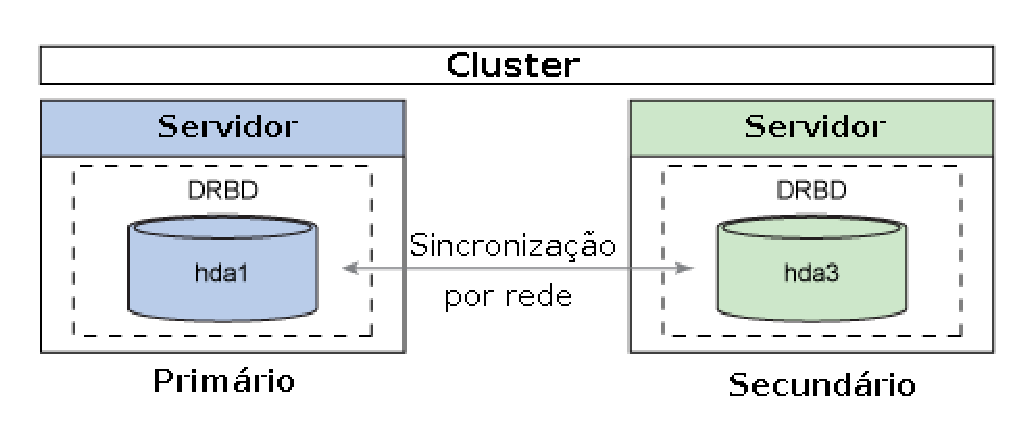
\includegraphics[width=300px]{img/drbd_basic.eps}
 }
 \caption{Exemplo do modelo \textit{master-slave} do \ac{DRBD}.}
 Fonte: \citet{jones2010}
 \label{fig:drbd_basic}
\end{figure}

O \ac{DRBD} pode ser configurado dos seguintes modos \cite{drbd}:
\begin{itemize}
 \item \textit{Single-primary} ou \textit{master-slave}: neste modo apenas um nó do \textit{cluster} pode ser o nó primário. Neste caso, somente
 o nó primário terá permissão para acessar o dispositivo, ou seja, somente ele poderá fazer operações de leitura e escrita. Já o nó 
 secundário terá apenas uma réplica dos dados;
 \item \textit{Dual-primary} ou \textit{dual-master}: neste modo existem dois nós primários, nos quais podem ser realizadas operações de leitura e 
 escrita de forma simultânea. Porém, este modo necessita de um sistema de arquivos compartilhados, sendo que neste caso pode ser utilizado, por
 exemplo, o \ac{GFS} \cite{gfs} ou o \ac{OCFS2} \cite{ocfs2}.
\end{itemize}

\subsubsection{GlusterFS}
\label{section:glusterfs}
O \textit{GlusterFS} \cite{glusterfs} é um sistema de arquivos distribuídos mantido pela \textit{Gluster community}. Esse \textit{software} 
utiliza estrutura de \textit{cluster} e seu principal objetivo é a escalabilidade, ou seja, este possui funcionalidades que facilitam o aumento
da capacidade do \textit{cluster} a partir da inclusão de novos nós.

Na Figura \ref{fig:glusterfs} tem-se um exemplo com dois nós, onde cada nó possui dois discos rígidos, que são denominados \textit{bricks}. 
A partir dos \textit{bricks} o \textit{GlusterFS} constrói um volume lógico que é disponibilizado através da rede para os clientes 
\textit{GlusterFS}. A organização destes \textit{bricks} vai depender do objetivo da aplicação, sendo que uma das formas é a replicação. Esses 
diferentes tipos de configurações serão detalhados a seguir.

\begin{figure}[h!]
 \centering
 \fcolorbox{black}{white}{
  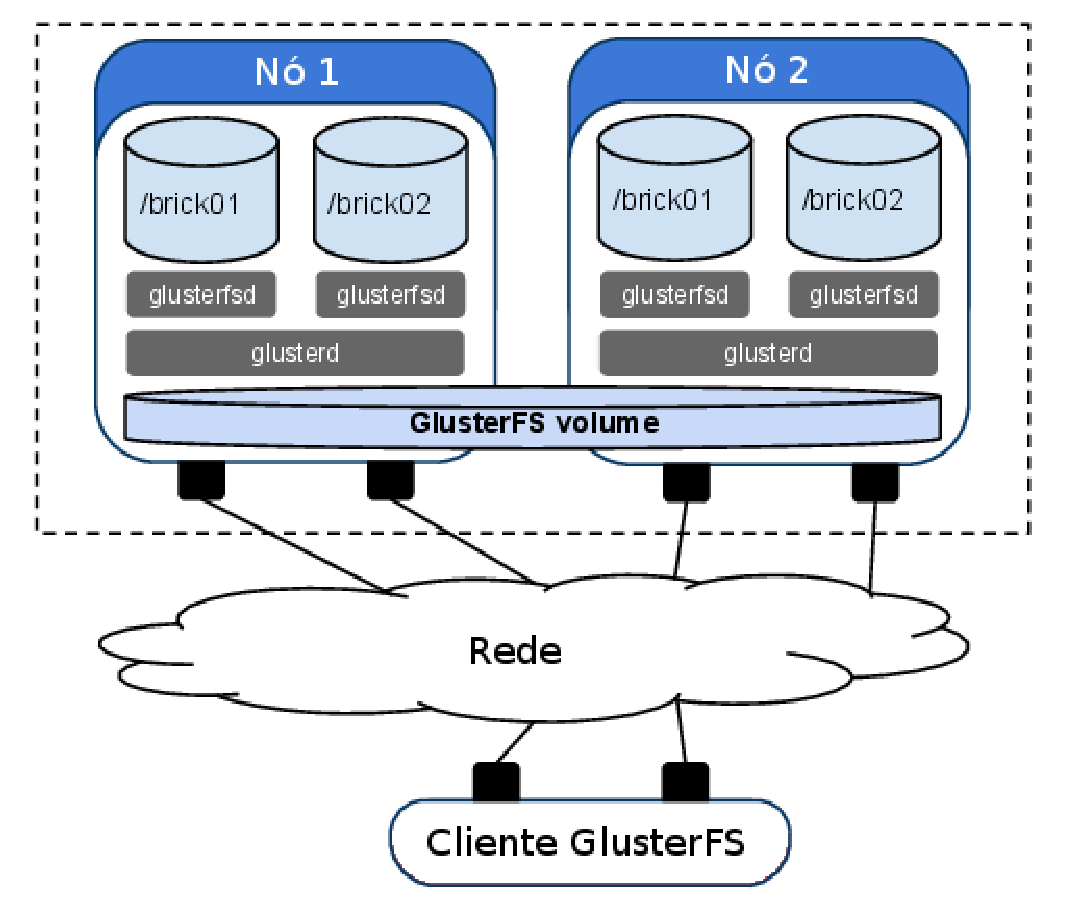
\includegraphics[width=280px]{img/glusterfs.eps}
 }
 \caption{Modelo do \textit{GlusterFS}.}
 Fonte: \citet{davies2013}
 \label{fig:glusterfs}
\end{figure}

O \textit{GlusterFS} suporta diferentes tipos de configurações de volumes, com as opções de distribuição e replicação de dados \cite{glusterfs}:
\begin{itemize}
 \item Volume distribuído: neste tipo os arquivos são distribuídos entre os diferentes \textit{bricks} dos nós. O objetivo deste tipo de 
 configuração é ampliar a capacidade de armazenamento. Desta forma, não tem-se preocupação com a redundância de dados, sendo que no caso de uma
 falha em um nó haverá uma perda de todos dados;
 \item Volume replicado: neste tipo os arquivos são replicados entre os \textit{bricks}, deste modo, tem-se uma redundância, ou seja, caso ocorra
 uma falha em um \textit{brick} não haverá perda de dados;
 \item Volume distribuído e replicado: este é a combinação dos dois tipos de volumes anteriores. Neste caso, é feita a distribuição 
 e a replicação dos arquivos entre os nós;
 \item Volume listrado: neste tipo ocorre a distribuição de um mesmo arquivo entre os \textit{bricks}, ou seja, um arquivo é dividido entre os
 \textit{bricks}, desta forma não ocorre replicação dos dados. Esse tipo é normalmente utilizado para armazenamento de arquivos muito grandes 
 e para balancear carga quando possuir muito acesso a disco;
 \item Volume distribuído e listrado: este tipo de volume é a combinação do distribuído e do listrado. Neste modo é feita a divisão do arquivo 
 entre \textit{bricks} distintos, sendo que estes são replicados.
\end{itemize}

\subsubsection{Rsync}
\label{section:rsync}
O \textit{Rsync} \cite{rsync} é um \textit{software} desenvolvido e mantido por \textit{Wayne Davison}. Esse \textit{software} provê uma rápida
transferência de arquivos, ou seja, ele faz o sincronização de arquivos em servidores transferindo dados de um servidor de origem para um de 
destino. A Figura \ref{fig:rsync} demonstra o funcionamento do \textit{Rsync}. Observa-se que no \textit{Rsync} tem-se uma replicação somente dos 
arquivos que ainda não foram atualizados ou que não existem no servidor de destino. Além disso, o \textit{Rsync} permite uma replicação completa, 
sendo que neste caso os arquivos já existentes são sobrescritos.

\begin{figure}[h!]
 \centering
 \fcolorbox{black}{white}{
  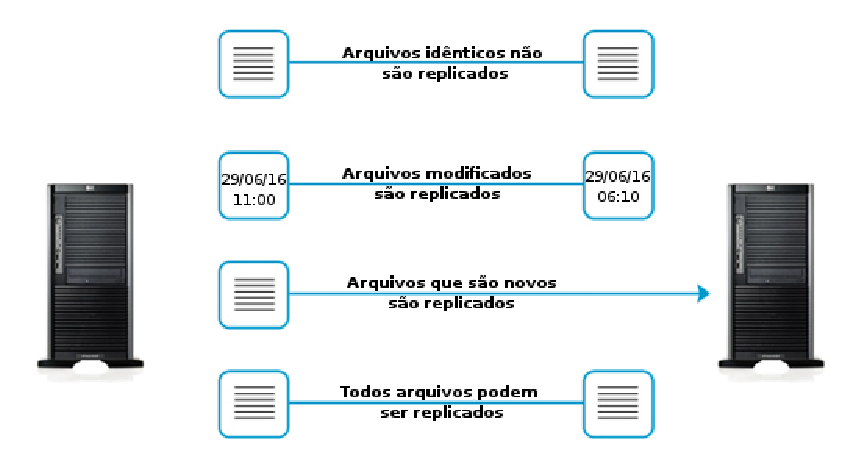
\includegraphics[width=370px]{img/rsync.eps}
 }
 \caption{Transferência de arquivos através do \textit{Rsync}.}
 Fonte: \citet{lopez2012}
 \label{fig:rsync}
\end{figure}

%Algoritmo \cite{tridgell98}

O \textit{Rsync} pode ser configurado como servidor, o que permite que vários clientes possam sincronizar os dados com ele. 
Além disso, a sincronização pode ser de cliente para cliente, utilizando como transporte o protocolo \ac{SSH} ou através de \textit{sockets}.
Destaca-se que o \textit{Rsync} não faz uma sincronização em tempo real, ou seja, ele faz a sincronização a partir de uma ação de um operador 
(execução de um comando).

% Ceph RBD
% Swift open stack
% https://wiki.freebsd.org/HAST

\subsubsection{Resumo e software de replicação adotado}
\label{section:replicacaoescolhido}

Na Tabela \ref{tab:replicacao} tem-se uma comparação entre as ferramentas citadas anteriormente. 
A ferramenta adotada para replicação de dados foi o \ac{DRBD}, pois permite a configuração \textit{dual-primary} e também \textit{master-slave}, 
além de suportar a replicação de discos das máquinas virtuais e fazer replicação a nível de bloco. Além disso, essa ferramenta permite a 
ressincronização dos dados de forma automática em caso de uma falha \cite{drbd}.

\begin{table}[h!]
\caption{Comparação ferramentas de replicação de dados.}
\label{tab:replicacao}
\begin{center}
\begin{tabular}{|l|p{3.5cm}|p{3.5cm}|p{2cm}|}\hline
\textbf{Características} & \textbf{DRBD} & \textbf{GlusterFS} & \textbf{Rsync} \\\hline
Integração com virtualização & Sim & Sim & Não \\\hline
Dual-primary & Sim & Sim & Não \\\hline
Replicação em tempo real & Sim & Sim & Não \\\hline
Nível de replicação & Bloco & Arquivo & Arquivo \\\hline
Número máximo de nós & 16 & 64 & Ilimitado \\\hline
Distribuições Linux & Suse, Debian, CentOS, Red Hat, Ubuntu & Debian, CentOS, Red Hat, Fedora, Ubuntu & Todas \\\hline
\end{tabular}
\end{center}
\end{table}

O \textit{GlusterFS} poderia ser utilizado, porém este faz uma replicação a nível de arquivo, sendo assim, não é adequada para uma 
solução de alta disponibilidade que utiliza-se de virtualização. 
E, por fim, o \textit{Rsync} não pode ser utilizado pois não executa uma replicação em tempo real, além de não ter sido desenvolvido para
ser utilizado em conjunto com a virtualização.

%Pode-se perceber que o \textit{Ceph RBD} não possui a opção de
%\textit{master-slave}. Esse \textit{software} necessita de um \textit{hardware} adicional para sua administração. 

%https://www.reddit.com/r/linux/comments/1qwarp/drbd_vs_glusterfs/
% glusterfs mais escalavel, simples de administrar
% drbd melhor eficiencia(acredito) nivel de bloco, confiavel(10 anos develop)

% drbd: 2 nodes na versão 8 e 16 nodes por stacking / 16 nodes na versão 9

% drbd dispositivo primário e secundário zaminhani2008
% Segundo (ELLENBERG, 2007), a partir da versão 8 do DRBD é possível que,
%dependendo da aplicação, a execução ocorra em todos os nós do cluster
%simultaneamente (Ativo/Ativo). Para tornar isso possível é necessária a
%utilização de um sistema de arquivos exclusivo para cluster, como o OCFS2 6 e o
%GFS 7 por exemplo. Como a abordagem deste trabalho é cluster de alta
%disponibilidade, a utilização do DRBD no modo Ativo/Ativo não será discutida.

% glusterfs https://raobharata.wordpress.com/2012/10/29/qemu-glusterfs-native-integration/
% melhor performace com disco utilizando protocolo gluster file=gluster://path/to

% ceph http://docs.ceph.com/docs/master/start/intro/
% necessita minimo 3 monitores com osd, outra para administração
% precisa openstack + nova
% http://www.server-world.info/en/note?os=Ubuntu_14.04&p=ceph
% https://elkano.org/blog/live-migration-openstack-ubuntu-14-04/

\subsection{Softwares para o gerenciamento de cluster}
\label{section:toolcluster}

Para ser possível implementar uma solução de alta disponibilidade é necessário organizar os servidores em uma estrutura de \textit{cluster},
sendo assim, é interessante a utilização de \textit{softwares} que facilitam o gerenciamento deste \textit{cluster}. Esses \textit{softwares} 
permitem detectar falhas em um nó, sendo elas de \textit{hardware} ou de serviços. Essas ferramentas são conhecidas como \ac{CRM}. 

Após a detecção de uma falha, os \textit{softwares} de gerenciamento de \textit{cluster} executam operações de \textit{failover} e 
\textit{failback}. O \textit{failover} é um processo no qual um servidor recebe os serviços que estavam executando no servidor que falhou. 
Já no \textit{failback} tem-se o retorno dos serviços para o servidor de origem quando este estiver disponível. Esse processo ocorre após o 
\textit{failover}, sendo que ele é opcional \cite{bassan2008}. Nas próximas seções tem-se uma breve descrição dos \textit{softwares} de 
gerenciamento de \textit{cluster} que foram estudados.

% \subsubsection{Ceph}
% \label{section:ceph}
% O \textit{Ceph} \cite{ceph} é uma ferramenta com foco no armazenamento de dados distribuídos. Esta ferramenta tem foco em \textit{cluster} 
% de armazenamento, sendo assim ela necessita de outra ferramenta para gerenciar as máquinas virtuais, como por exemplo \textit{OpenStack} 
% \cite{openstack}. Sua arquitetura é composta por um nó administrador, onde tem-se a gerência do \textit{cluster}, e no mínimo dois 
% nós, sendo um para o armazenamento (\textit{Ceph OSD}) e um para o monitoramento (\textit{Ceph Monitor}) e o processamento (\textit{Ceph MDS}) \cite{ceph}.

\subsubsection{Ganeti}
\label{section:ganeti}
O \textit{Ganeti} \cite{ganeti} é um \textit{software} desenvolvido pelo \textit{Google}. Esse \textit{software} é um gerenciador de 
\textit{cluster} de virtualização. Ele foi desenvolvido especificamente para ambientes de virtualização e suporta os hipervisores 
\ac{KVM} \cite{kvm} e \textit{Xen} \cite{xen}. 

Na Figura \ref{fig:ganeti_arquitetura} tem-se um exemplo de um \textit{cluster} com a arquitetura do \textit{Ganeti}, sendo que este 
\textit{cluster} é composto por um nó \textit{master}, que armazena as configurações e gerencia o \textit{cluster}, e um nó 
\textit{master candidate}, para o caso do nó \textit{master} falhar. Além disso, a arquitetura é formada por vários nós \textit{slaves}. 
Destaca-se que no \textit{Ganeti} todos os nós são responsáveis por prover o ambiente de virtualização e armazenar os dados das \acp{VM}, 
sendo que cada nó pode possuir uma ou mais instâncias de \acp{VM}. Em cada instância das \acp{VM} configura-se dois nós: o nó primário, que a 
instância executará inicialmente; e o nó secundário, que será utilizado no caso do nó primário falhar.
Além disso, as instâncias das \acp{VM} também podem ser migradas de um nó para outro de forma manual. 

\begin{figure}[h!]
 \centering
 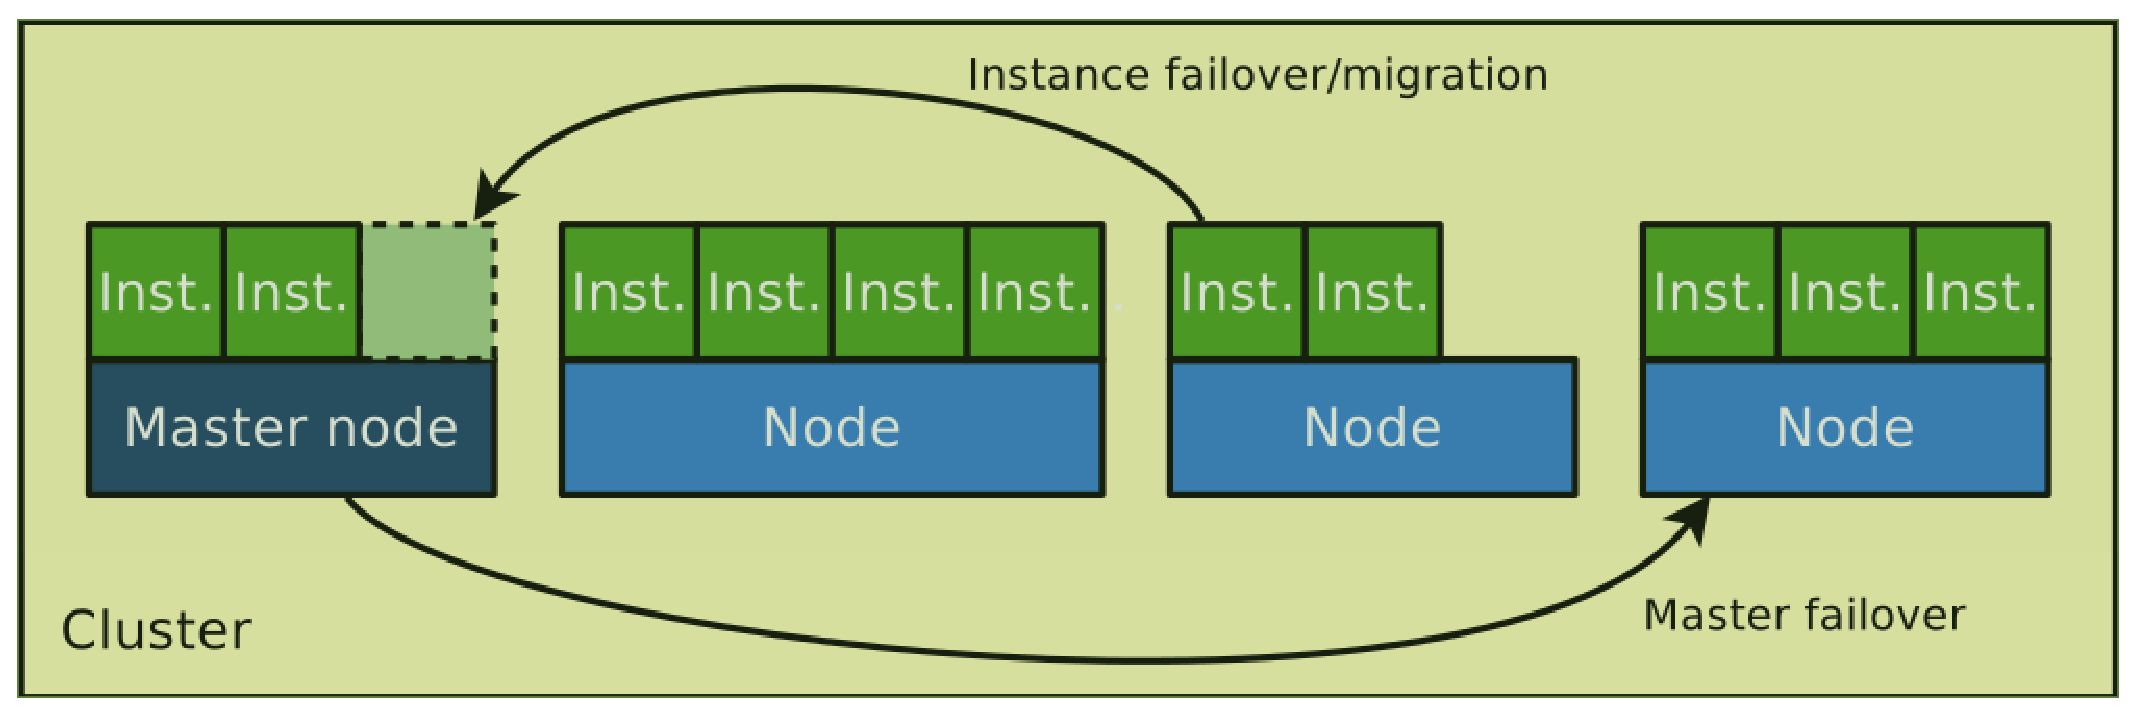
\includegraphics[width=380px]{img/ganeti_arquitetura.eps}
 \caption{Arquitetura do \textit{Ganeti}.}
 Fonte: \citet{carvalho2011}
 \label{fig:ganeti_arquitetura}
\end{figure}

De forma resumida, as principais funcionalidades do \textit{Ganeti} são \cite{ganeti}:
\begin{itemize}
 \item Criação de instâncias de \acp{VM};
 \item Gerenciamento do armazenamento das instâncias;
 \item Iniciar e finalizar instâncias, além de efetuar a migração entre os nós.
\end{itemize}

% ganeti pode ser usado com ceph rdb (RADOS Cluster), ou drbd, ou gluster

\subsubsection{Heartbeat}
\label{section:heartbeat}
O \textit{Heartbeat} é um subprojeto do \textit{Linux-HA} \cite{linuxha}, que desenvolve soluções de alta disponibilidade.
Esse subprojeto é uma aplicação que envia pacotes \textit{keepalive \ac{UDP}}, através da rede, para outras aplicações \textit{Heartbeat}. 
Esses pacotes possuem como objetivo verificar se uma aplicação está ativa.
Destaca-se que esse \textit{software} pode ser utilizado para alta disponibilidade em ambientes de virtualização \cite{reis2009}.

Na Figura \ref{fig:heartbeat} tem-se o \textit{Heartbeat} executando em dois servidores sobre as interfaces de rede dedicadas (identificadas na 
figura como \textit{ethX}).
Neste caso, se o nó secundário deixar de receber os sinais do nó primário, este irá tornar-se o nó primário, e iniciará o processo de 
\textit{failover}. 
%com isso, ele receberá o \ac{IP} virtual (\textit{192.168.50.3}) e iniciará os serviços previamente configurados.
\begin{figure}[h!]
 \centering
 \fcolorbox{black}{white}{
  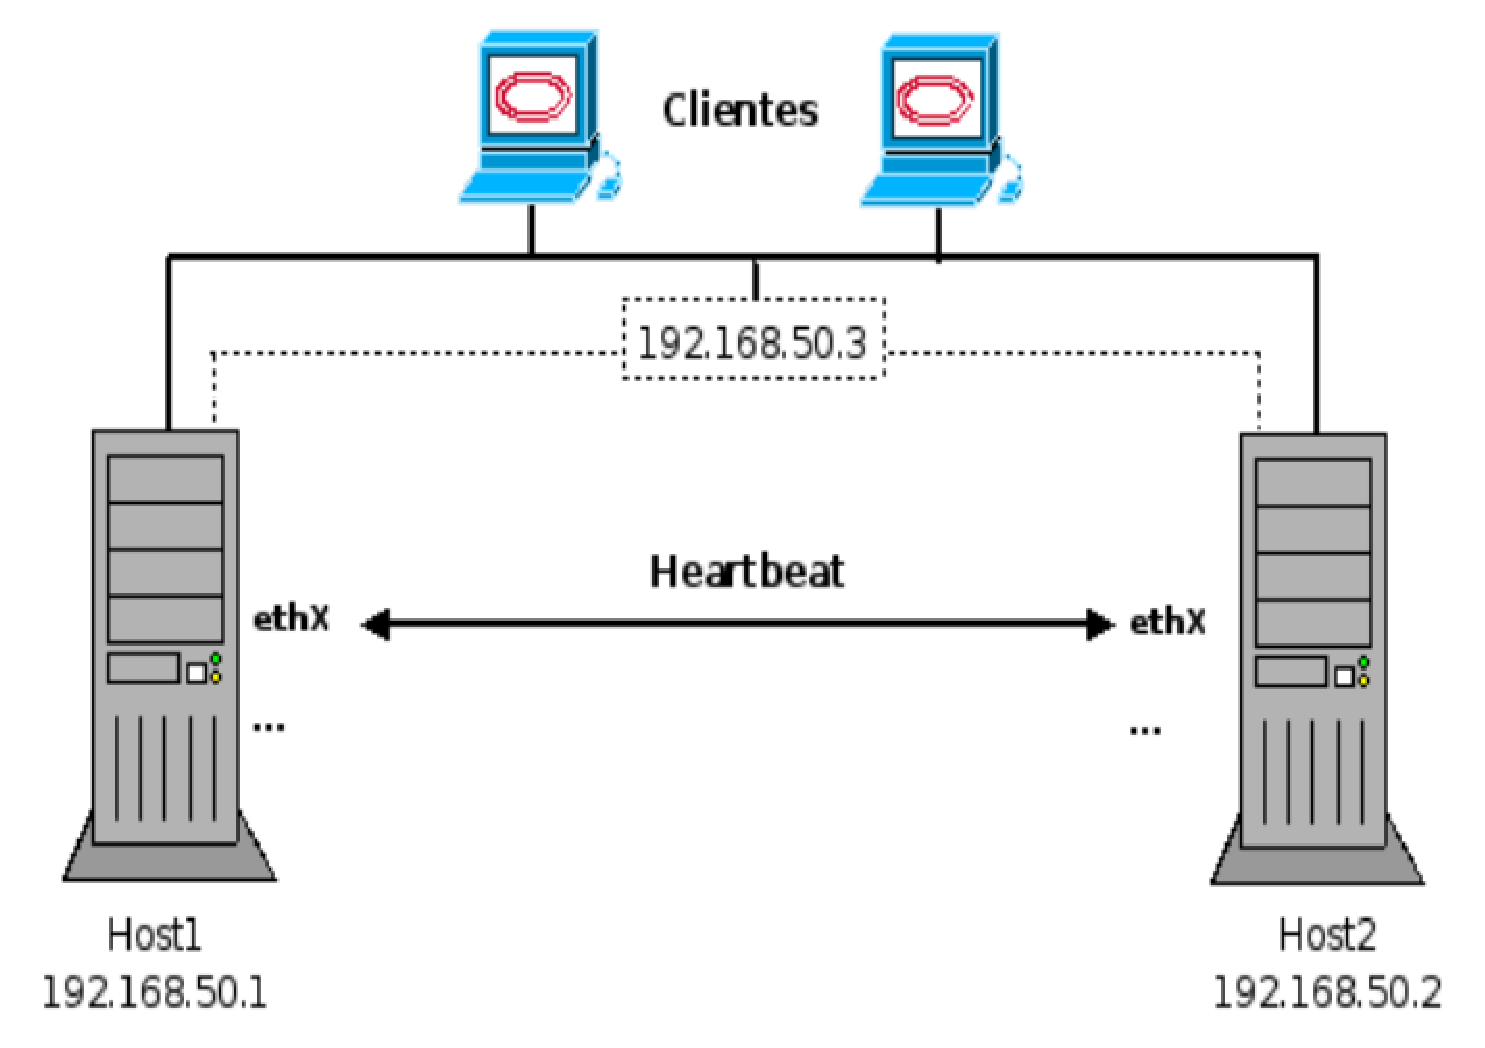
\includegraphics[width=300px]{img/heartbeat.eps}
 }
 \caption{Arquitetura do \textit{Heartbeat}.}
 Fonte: \citet{zaminhani2008}
 \label{fig:heartbeat}
\end{figure}

De forma resumida, as principais funcionalidades do \textit{Heartbeat} são \cite{clusterlabs}:
\begin{itemize}
 \item Enviar mensagens entre os nós para a detecção de falhas;
 \item Efetuar os processos de \textit{failover} e \textit{failback};
 \item Iniciar e finalizar serviços nos nós;
\end{itemize}

%exemplo de implementacao heartbeat com virtualizacao = \cite{reis2009}

\subsubsection{Pacemaker}
\label{section:pacemaker}
O \textit{Pacemaker} \cite{pacemaker} é um projeto de código aberto mantido pela \textit{ClusterLabs}, e teve origem com a necessidade de 
aperfeiçoar o \textit{Heartbeat} \cite{heartbeat}. 
O \textit{Pacemaker} pode ser definido como um \textit{software} de recuperação de falhas a nível de serviço \cite{perkov2011}. 

Esse \textit{software} é utilizado juntamente com outro \textit{software} que fazem registro dos nós e troca de mensagens entre os nós do 
\textit{cluster}, sendo que os \textit{softwares} que podem ser integradas com o \textit{Pacemaker} são \cite{pacemaker}:
\begin{itemize}
 \item \textit{Corosync} \cite{corosync}: derivou do projeto \textit{OpenAIS} e é responsável pelo processo de registro dos nós e pelo processo 
 de \textit{failover};
 %bloqueios distribuídos (utilizados para implementar \ac{LVM} \cite{lvm}, \ac{GFS}, e \ac{OCFS2}). 
 \item \textit{Heartbeat}: responsável pelo envio de mensagens entre os nós do \textit{cluster}, além de iniciar e finalizar serviços.
\end{itemize}
% outras ferramentas cMAN e Apache Qpid

%Modelos Active/Passive, N+1, N TO N, Split Site

Na Figura \ref{fig:pacemaker_tools} tem-se a arquitetura do \textit{Pacemaker}. Como pode ser observado na camada inferior tem-se os nós do 
\textit{cluster}. Na camada superior tem-se o \textit{software} de envio de mensagens e acima deste tem-se o \textit{Pacemaker}. 
Por fim, tem-se os serviços, que serão executados no \textit{cluster}.

\begin{figure}[h!]
 \centering
 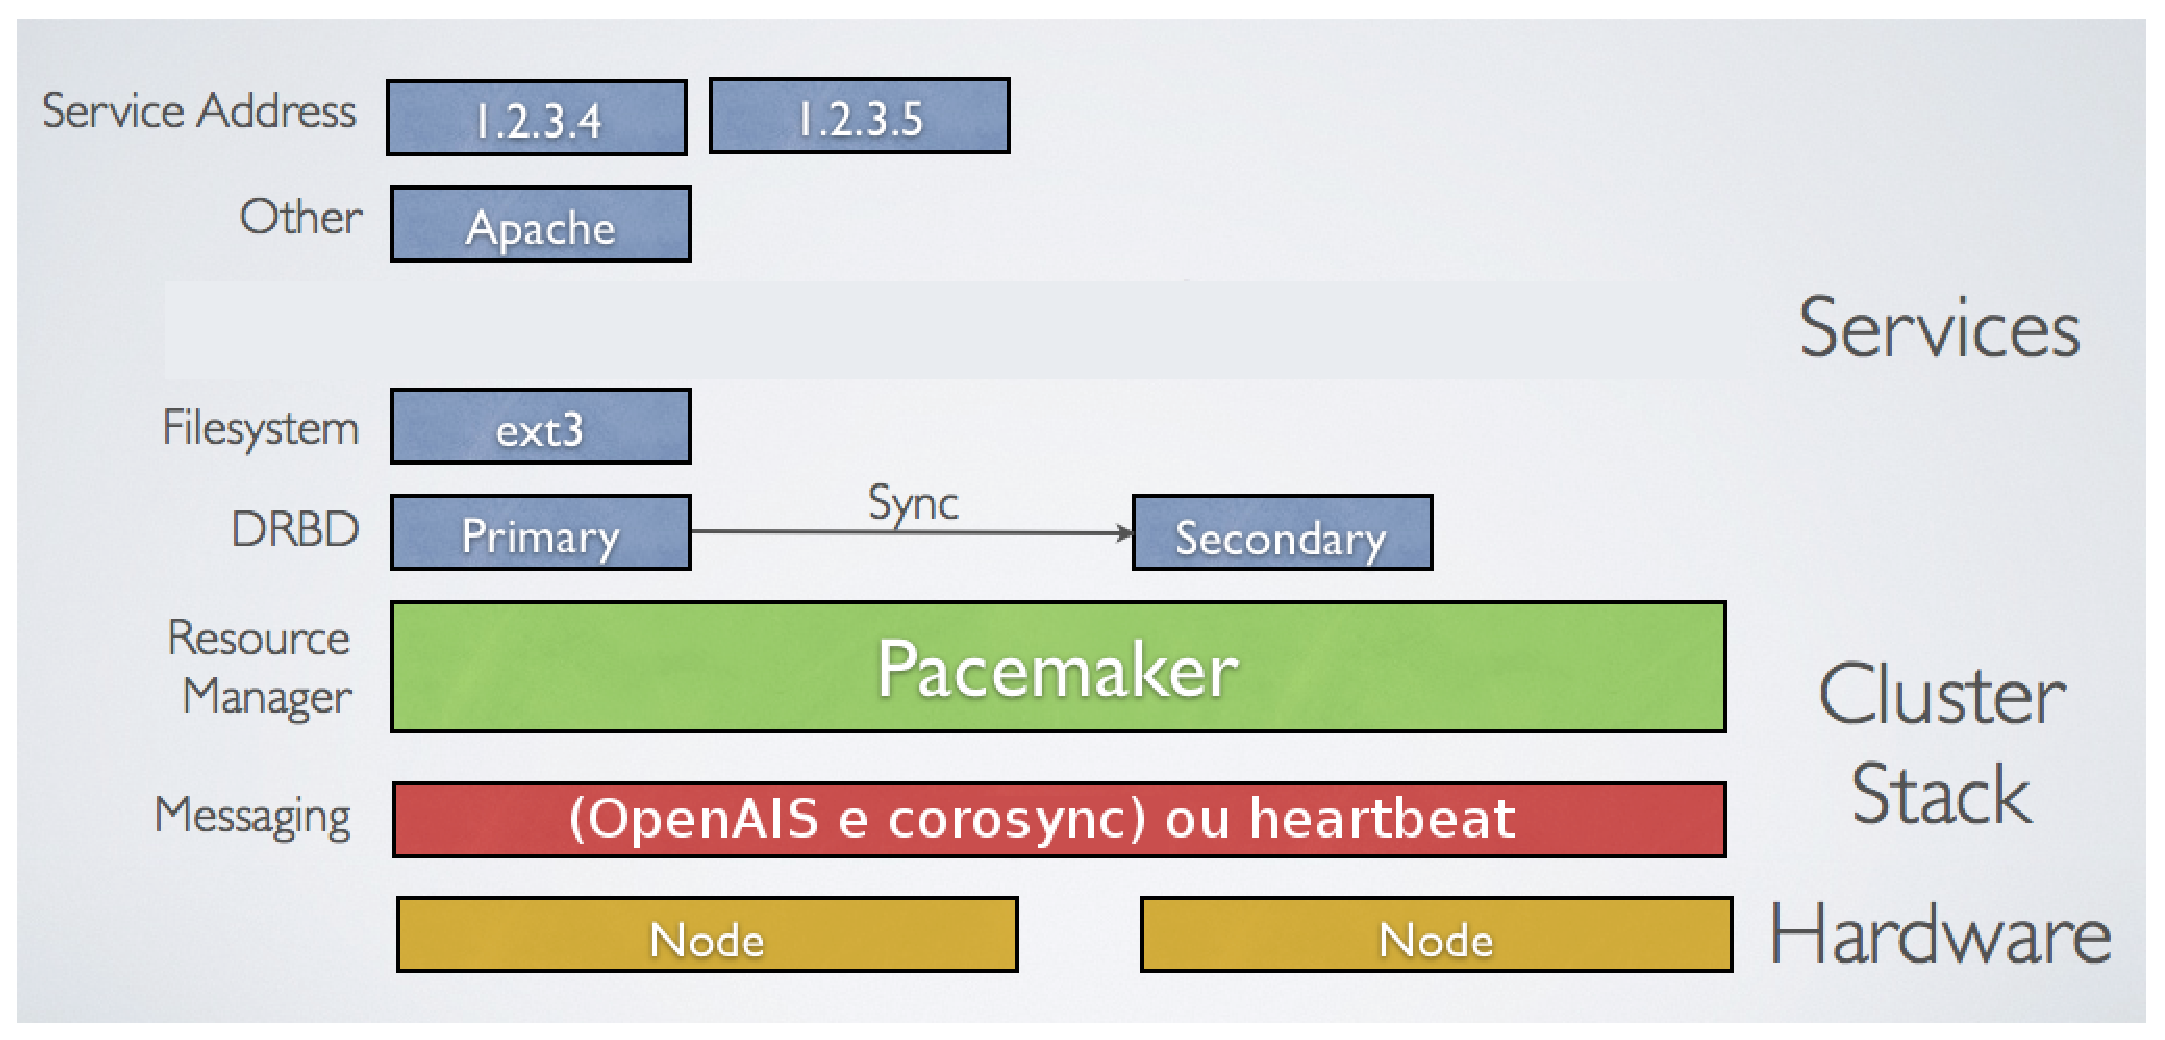
\includegraphics[width=350px]{img/pacemaker_tools.eps}
 \caption{Exemplo da arquitetura do \textit{Pacemaker}.}
 Fonte: \citet{pacemaker}
 \label{fig:pacemaker_tools}
\end{figure}

Entre as principais funcionalidades do \textit{Pacemaker} destaca-se:
\begin{itemize}
 \item Iniciar e finalizar os serviços dos nós do \textit{cluster}. Esses serviços podem ser desde um servidor \textit{web}, uma interface de 
 rede, ou até uma máquina virtual;
 \item Replicação de configuração do \textit{cluster} para todos os nós de forma transparente. Desta forma, a configuração do \textit{cluster} 
 pode ser alterada em qualquer nó;
 \item Eleição de um nó como primário. No caso de uma falha neste nó, um outro será eleito primário de forma automática.
\end{itemize}

No \textit{Pacemaker} os serviços são denominados recursos (\textit{resources}), esses recursos são monitorados, iniciados e parados.
Pode-se criar dependências e ordem entre esses recursos, para que esses sejam iniciados em uma determinada sequencia. O \textit{Pacemaker} 
também pode ser configurado para fazer o \textit{failover}, desta forma caso ocorra uma falha em um nó, esse fará a inicialização dos serviços 
em um nó secundário. Além disso, essa ferramenta também faz a recuperação de um recurso que, por alguma falha, parou de executar, por exemplo, 
se ocorrer algum erro interno em um \textit{software} que fornece algum serviço e este for interrompido, o \textit{Pacemaker} tentará iniciá-lo
novamente.

% Corosync provides pacemaker:
% a mechanism to reliably send messages between nodes,
% notifications when machines appear and disappear
% a list of machines that are up that is consistent throughout the cluster 
% Heartbeat provides:
% a mechanism to reliably send messages between nodes,
% notifications when machines appear and disappear
% a list of machines that are up that is consistent throughout the cluster 
% --
% http://serverfault.com/questions/269831/relation-between-heartbeat-openais-corosync
% well i reached answer on myself! clustering include two part:
% 1.cluster resource management
% 2.infrastructure with massaging layer
% legacy heartbeat is broken into heartbeat message layer and pacemaker so pacemaker is CRM.
% and we have two option on message layer:heartbeat,openais. openais/corosync is preferred as: http://comments.gmane.org/gmane.linux.
%highavailability.user/32355
% There are, however, features in Pacemaker that require OpenAIS which will work only with Corosync, not Heartbeat. Those features are concerned 
% with the distributed lock managers used by cLVM (but not regular LVM), GFS/GFS2, and OCFS2. If you need that functionality, you must select 
% OpenAIS/Corosync. If you do not, you're free to choose.
% as: http://www.clusterlabs.org/wiki/FAQ
% Originally Corosync and OpenAIS were the same thing. Then they split into two parts... the core messaging and membership capabilities are now 
% called Corosync, and OpenAIS retained the layer containing the implementation of the AIS standard.
% Pacemaker itself only needs the Corosync piece in order to function, however some of the applications it can manage (such as OCFS2 and GFS2) 
% require the OpenAIS layer as well.
% so i went to openais/corosync and integrate it with pacemaker.
% --
% There are, however, features in Pacemaker that require OpenAIS which
% will work only with Corosync, not Heartbeat. Those features are
% concerned with the distributed lock managers used by cLVM (but not
% regular LVM), GFS/GFS2, and OCFS2. If you need that functionality, you
% must select OpenAIS/Corosync.
% 
% Pacemaker itself only needs the Corosync piece in order to function, however some of the applications it can manage 
% (such as OCFS2 and GFS2) require the OpenAIS layer as well. 

\subsubsection{Resumo e software de gerenciamento adotado}
\label{section:gerenciadorescolhido}

Na Tabela \ref{tab:clusterger} tem-se uma comparação dos \textit{softwares} de gerenciamento de \textit{cluster}. 
O \textit{software} escolhido para gerenciar o ambiente foi o \textit{Pacemaker}, pois este possui todos os requisitos para a criação de um 
\textit{cluster} de alta disponibilidade utilizando virtualização. A principal característica disponível neste é o \textit{failover} automático
dos nós, que não encontra-se disponível nas demais ferramentas. Além disso, essa ferramenta possibilita a migração em tempo real, 
e é o único que possui o sincronismo de configuração entre todos os nós. 
%Destaca-se que o \textit{Pacemaker} é indicado no site do \ac{DRBD} para compor um \textit{cluster} de alta disponibilidade \cite{drbd}.

\begin{table}[h!]
\caption{Comparação entre ferramentas de gerenciamento de \textit{cluster}.}
\label{tab:clusterger}
\begin{center}
\begin{tabular}{|p{4cm}|p{2cm}|p{3.5cm}|p{3.5cm}|}\hline
\textbf{Características} & \textbf{Ganeti} & \textbf{Heartbeat} & \textbf{Pacemaker} \\\hline
Suporte nativo a virtualização & Sim & Não & Sim \\\hline
Migração de \acp{VM} em tempo real & Sim & Não & Sim \\\hline
Failover e failback automáticos & Não & Não & Sim \\\hline
Sincronismo de configuração entre os nós & Não & Não & Sim \\\hline
Distribuições Linux & Todas & Red Hat, CentOS, Fedora, Suse, Debian, Ubuntu & Red Hat, CentOS, Fedora, Suse, Debian, Ubuntu \\\hline
\end{tabular}
\end{center}
\end{table}

O \textit{software} \textit{Ganeti} não se mostrou adequado pois não possui suporte para fazer um \textit{failover} de forma automática. 
%Essa ferramenta não possui foco na disponibilidade, mas sim na segurança dos dados, pois os dados ficam replicados e podem ser recuperados de forma manual. 
Seria possível também implementar uma solução de alta disponibilidade com a ferramenta \textit{Heartbeat}. Porém, neste caso seria necessário 
criar um conjunto de \textit{scripts} para a migração das máquinas virtuais.

% Pode-se observar que o \textit{software} \textit{Ceph} possui suporte apenas para a detecção e recuperação a nível de nó. De fato, esse 
% \textit{software} tem foco em \textit{cluster} de armazenamento, desta forma necessitando de outra ferramenta para gerenciar a migração de 
% máquinas virtuais. Além disso, essa ferramenta necessita de um \textit{hardware} especifico para administração do \textit{cluster}.


\section{Implementação}
\label{section:implementacao}

%Para implementação desta solução foram necessários dois servidores físicos, sendo que a configuração ideal de cada servidor é de 
%real = 11 \textit{cores} de processamento, 12 GB de memória \ac{RAM} e 156 GB de disco rígido
%12 \textit{cores} de processamento, 14 GB de memória \ac{RAM} e 180 GB de disco rígido. Essa configuração foi calculada a partir da soma dos 
%recursos das máquinas virtuais que atualmente abrangem os serviços que foram considerados críticos, observa-se que tais recursos de 
%\textit{hardware} já encontravam-se disponíveis, sendo necessário somente efetuar uma reorganização das máquinas virtuais. Com essa solução, 
%caso ocorra alguma falha em um servidor, as máquinas virtuais serão transferidas para o outro servidor.

O ambiente foi configurado na forma de um \textit{cluster}, o qual é composto por dois servidores com requisitos de configuração 
de 12 \textit{cores} de processamento, 14 GB de memória \ac{RAM} e 180 GB de disco rígido.
%real = 11 \textit{cores} de processamento, 12 GB de memória \ac{RAM} e 156 GB de disco rígido
Essa configuração foi calculada a partir da soma dos recursos das máquinas virtuais que abrangem os serviços que foram considerados críticos. 
Observa-se que tais recursos de \textit{hardware} já encontravam-se disponíveis, sendo necessário somente efetuar uma reorganização 
das máquinas virtuais. Destaca-se que a configuração também inclui 2 GB de memória \ac{RAM} e 24 GB de disco para cada sistema operacional hóspede.

Além disso, optou-se por utilizar o mesmo sistema operacional e o mesmo hipervisor que já foram adotados atualmente na empresa, o sistema 
\textit{Ubuntu 14.04 \ac{LTS}} e o \ac{KVM} \cite{kvm}, respectivamente. O processo de instalação e de configuração encontra-se no 
Apêndice \ref{ap:confos} e \ref{ap:confvirt}.

A estrutura física adotada está representada na Figura \ref{fig:projeto_fisico} (a). Como pode-se observar os dois servidores encontram-se 
conectados a um \textit{switch} através de dois cabos UTP, de forma a implementar uma redundância do cabeamento. Além disso, manteve-se o 
\textit{link aggregation} e utilizou-se uma \textit{bridge}\footnote{\textit{Bridges}, também conhecidas como pontes, são meios que fazem a 
conexão entre \textit{LANs}, e operam na camada de enlace de dados.} para incluir as máquinas virtuais à rede. 
Os detalhes da configuração de rede estão localizados no Apêndice \ref{ap:confrede}.
Na Figura \ref{fig:projeto_fisico} (b) tem-se a imagem dos servidores, o primeiro é o Nó 1 (\textit{Brina}), que é um 
\textit{Dell PowerEdge 2950}, e o segundo servidor é o Nó 2 (\textit{Piova}), que é um \textit{Dell PowerEdge R410}.

\begin{figure}[h!]
 \centering
 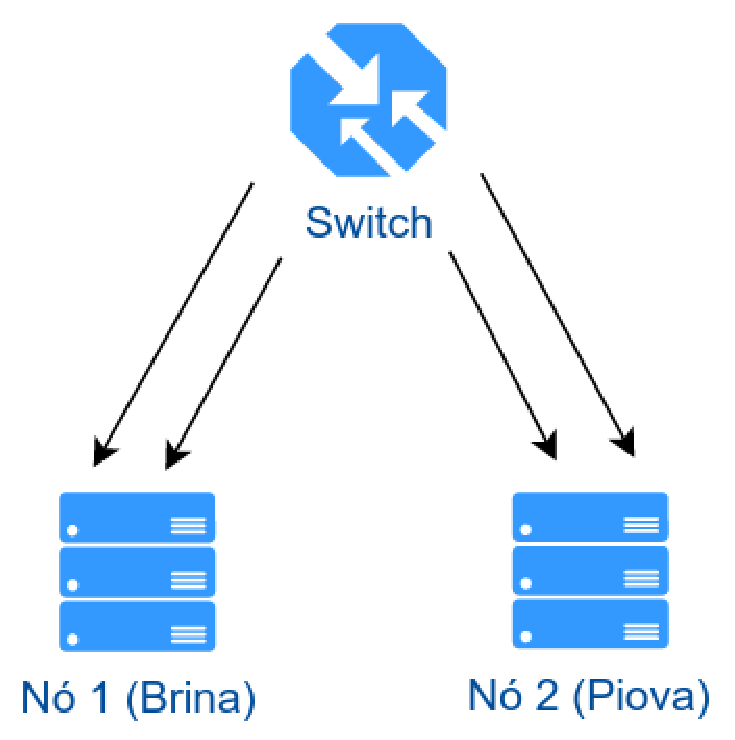
\includegraphics[width=450px]{img/projeto_fisico.eps}
 \caption{Estrutura física.}
 \label{fig:projeto_fisico}
\end{figure}

A estrutura lógica dos servidores juntamente com as máquinas virtuais e seus respectivos serviços são apresentados na Figura 
\ref{fig:projeto_estrutura}. Para a replicação de dados foi utilizado o \textit{software} \ac{DRBD}, que foi configurado no modo 
\textit{dual-master} onde os dois nós são configurados como primários. Para tal configuração é necessário utilizar um sistema de arquivos 
distribuídos para um acesso compartilhado dos dados, sendo que o \textit{software} adotado foi o \ac{OCFS2} \cite{ocfs2}. 
Os detalhes da instalação e da configuração de disco, \ac{DRBD} e sistema de arquivos estão detalhadas no Apêndice \ref{ap:confdisco}. 
Já para o gerenciamento do \textit{cluster} e das \acp{VM} utilizou-se o \textit{software} \textit{Pacemaker}. 
Mais especificamente esse é o \textit{software} responsável pelo monitoramento e pela migração das \acp{VM} entre os nós.

\begin{figure}[h!]
 \centering
 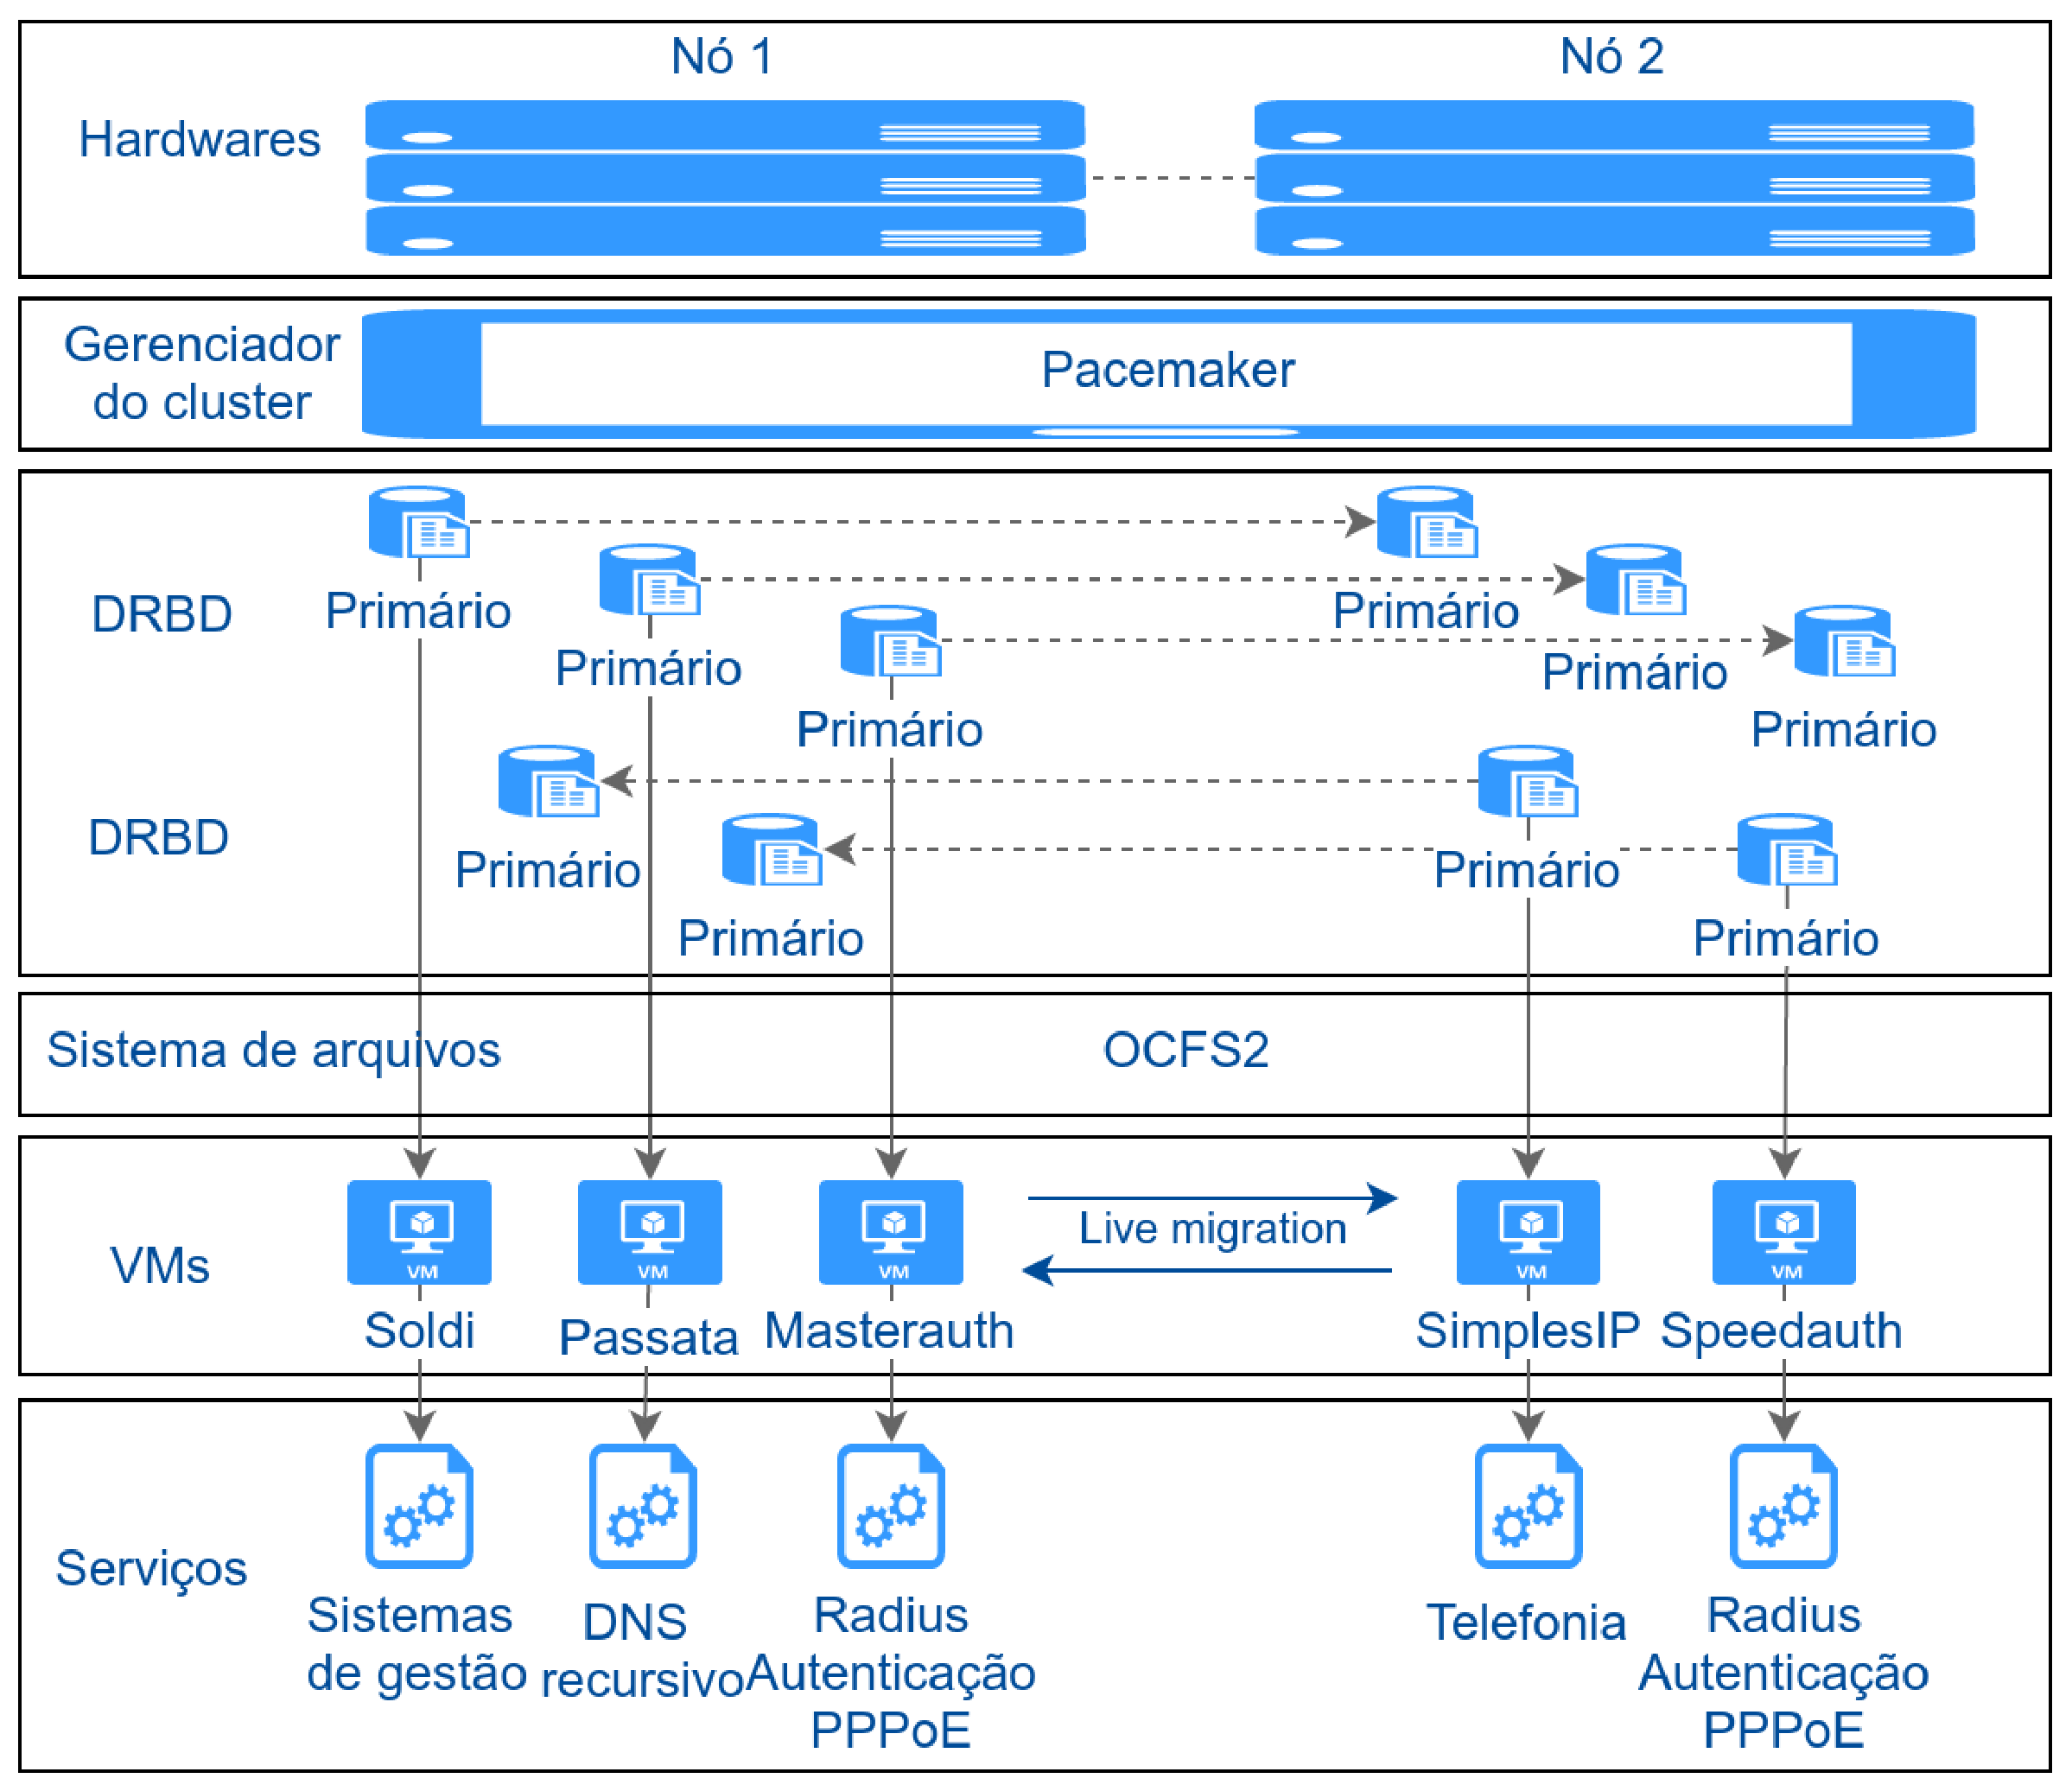
\includegraphics[width=350px]{img/projeto_estrutura.eps}
 \caption{Estrutura do \textit{cluster}.}
 \label{fig:projeto_estrutura}
\end{figure}

%drbd
% O \ac{DRBD} será configurado no modo \textit{master-slave}, sendo que para cada disco das máquinas virtuais será criado um dispositivo de 
% replicação \ac{DRBD}. E para utilizar esse dispositivo como disco de uma máquina virtual será criado um volume lógico 
% \ac{LVM}\footnote{LVM é uma ferramenta de código aberto que possibilita a manipulação de discos rígidos, através da criação de grupos de volumes 
% e volumes lógicos para \textit{Linux}.} \cite{lvm}. 

Os serviços foram distribuídos entre os nós dos \textit{cluster}, sendo que no Nó 1 foram instalados os serviços de sistemas de gestão, 
\ac{DNS} recursivo e autenticação \ac{PPPoE}. Já no Nó 2 foram instalados os serviços de telefonia e autenticação \ac{PPPoE}.
No caso de falha em um nó, os serviços serão inicializados no outro nó disponível. O detalhamento da configuração do \textit{Pacemaker} 
estão disponíveis no Apêndice \ref{ap:confpacemaker}.


\section{Considerações finais}

Neste capítulo foram selecionadas e apresentadas as ferramentas para implementação de alta disponibilidade, sendo selecionadas através de uma
metodologia juntamente com algumas características criadas. Além disso, foi apresentada a implementação da solução de alta disponibilidade, que é
composta por dois servidores físicos, onde foram configuradas máquinas virtuais contendo os serviços críticos da empresa. 

No próximo capítulo serão descritos os testes criados, apresentado os resultados obtidos e construida a conclusão final do trabalho. 
Com isso, pretende-se comprovar a eficácia do projeto e do ambiente criado.
